\documentclass[lualatex, a4paper, ja=standard]{bxjsarticle}

\usepackage{luatexja}
\usepackage{graphicx}
\usepackage{amsmath, amssymb}
\usepackage{syntax}
\usepackage{fancyvrb}
\usepackage{url}
\usepackage{tikz}

% \setlength{\grammerparsep}{}
\setlength{\grammarindent}{16em}

\setpagelayout*{margin=20truemm}

\title{2022年度 コンパイラ実験 最終レポート}
\author{氏名:  \\ 学生番号: }

\begin{document}
\maketitle

\section{概要}
Flex,Bison を用いて,独自の言語を
maps で動作するアセンブリ言語に変換するコンパイラを作成する.

コンパイラのソースコードはGitHub
\footnote{\url{https://github.com/AAAR-Salmon/experiment-compiler/tree/compiler}}
にある.

\section{作成する言語の概要}

\subsection{文法}

この言語は次のような文法を持つ.
ただし,$\langle\mathit{identifier}\rangle$ は
正規表現 \verb/[a-zA-Z][a-zA-Z0-9]*/ に,
$\langle\mathit{number}\rangle$ は
正規表現 \verb/[0-9]+/ にマッチするトークンである.
また,\verb'#' から行末までをコメントとして扱う.

\begin{grammar}
<program> ::=
  <declarations> <statements>

<declarations> ::=
  <declaration-statement> <declarations> \alt
  <declaration-statement>

<declaration-statement> ::=
  `define' <identifier> `;' \alt
  `array' <identifier> `[' <number> `]' `;'

<statements> ::=
  <statement> <statements> \alt
  <statement>

<statement> ::=
  <assign-statement> \alt
  <loop-statement> \alt
  <branch-statement>

<assign-statement> ::=
  <reference> `=' <expression> `;'

<loop-statement> ::=
  `while' `(' <expression> `)' `{' <statements> `)'

<branch-statement> ::=
  `if' `(' <expression> `)' `{' <statements> `}' \alt
  `if' `(' <expression> `)' `{' <statements> `}' `else' `{' <statements> `}'

<reference> ::=
  <identifier> \alt
  <identifier> `[' <expression> `]'

<expression> ::=
  <expression> `and' <conditional-expression> \alt
  <expression> `or' <conditional-expression> \alt
  `not' <conditional-expression> \alt
  <conditional-expression>

<conditional-expression> ::=
  <additional-expression> `==' <additional-expression> \alt
  <additional-expression> `!=' <additional-expression> \alt
  <additional-expression> `<' <additional-expression> \alt
  <additional-expression> `<=' <additional-expression> \alt
  <additional-expression> `>' <additional-expression> \alt
  <additional-expression> `>=' <additional-expression> \alt
  <additional-expression>

<additional-expression> ::=
  <additional-expression> `+' <multiplicational-expression> \alt
  <additional-expression> `-' <multiplicational-expression> \alt
  <multiplicational-expression>

<multiplicational-expression> ::=
  <multiplicational-expression> `*' <primitive-expression> \alt
  <multiplicational-expression> `/' <primitive-expression> \alt
  <multiplicational-expression> `%' <primitive-expression> \alt
  <primitive-expression>

<primitive-expression> ::=
  <reference> \alt
  <number> \alt
  `(' <expression> `)'
\end{grammar}

\subsection{受理するプログラムの例}

以下に示すプログラムは必ずしも正常にコンパイルされるものではない.

\begin{Verbatim}[frame=lines, numbers=left]
define s;
define i;

s = 0;
i = 1; while (i <= 10) {
  s = s + i;
  i = i + 1;
}
\end{Verbatim}

\begin{Verbatim}[frame=lines, numbers=left]
array fib[20];
define i;

fib[0] = 0;
fib[1] = 1;
i = 2; while (i < 20) {
  fib[i] = fib[i-1] + fib[i-2];
}
\end{Verbatim}

\begin{Verbatim}[frame=lines, numbers=left]
define in1;
define in2;
define inc;
define outs;
define outc;

# set input here
in1 = 0;
in2 = 1;
inc = 1;

# outs = (in1 xor in2) xor inc
outs = (in1 and (not in2)) or ((not in1) and in2);
outs = (outs and (not inc)) or ((not outs) and inc);

outc = ((in1 and in2) or (in1 and inc)) or (in2 and inc);
\end{Verbatim}

\section{コード生成}

Bisonプログラムによって作成した抽象構文木(AST)を辿って生成する.

\subsection{メモリ領域}

0x00000000 から大きいアドレスがプログラムの初期化部領域,
0x00001000 から大きいアドレスがプログラムコード部領域,
0x10008000 から大きいアドレスがグローバル変数領域,
0x80000000 から\textbf{小さい}アドレスが計算用スタック領域である.

2領域がオーバーラップしたときの動作は保証されない.

\subsection{レジスタ}

このコンパイラにおける各レジスタの用途を,
表 \ref{tab:register} に示す.
示されていないレジスタは未使用である.

\begin{table}[b]
  \centering
  \caption{レジスタの用途}
  \label{tab:register}
  \begin{tabular}{|rl|l|} \hline
    レジスタ番号 & レジスタ名 & 用途 \\ \hline\hline
    0  & \$zero & 値 $0$ の参照 \\
    1  & \$at   & (アセンブラのために予約) \\
    2  & \$v0   & 式の評価値 \\
    3  & \$v1   & 式の評価値 \\
    4  & \$a0   & (関数のために予約) \\
    8  & \$t0   & 変数アドレスの計算用 \\
    26 & \$k0   & (OSのために予約) \\
    27 & \$k1   & (OSのために予約) \\
    28 & \$gp   & グローバル変数領域の先頭アドレス \\
    29 & \$sp   & 計算用スタックのトップアドレス \\
    30 & \$fp   & (関数のために予約) \\
    31 & \$ra   & (関数のために予約) \\ \hline
  \end{tabular}
\end{table}

\subsection{算術式のコード生成}

式のASTは,not演算子を除き,
図\ref{fig:ast-expression} のいずれかの形を取る.

続く小節ではそれぞれの場合のコード生成を説明する.
not演算子については取る式が1つであることを除き
二項演算と大きくは変わらないため省略する.

\begin{figure}[t]
  \centering
  \begin{tabular}{cccc}
    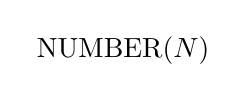
\begin{tikzpicture}
      \node{ NUMBER($N$) };
    \end{tikzpicture} &
    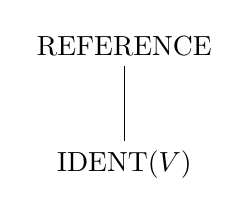
\begin{tikzpicture}
      \node{ REFERENCE }
        child { node { IDENT($V$) } };
    \end{tikzpicture} &
    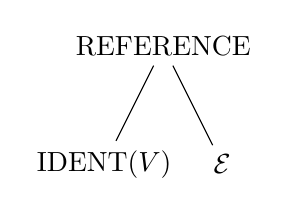
\begin{tikzpicture}
      \node{ REFERENCE }
        child { node { IDENT($V$) } }
        child { node { $\mathcal{E}$ } };
    \end{tikzpicture} &
    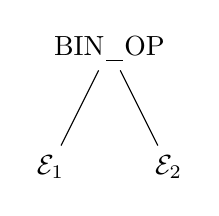
\begin{tikzpicture}
      \node{ BIN_OP }
        child { node { $\mathcal{E}_1$ } }
        child { node { $\mathcal{E}_2$ } };
    \end{tikzpicture} \\
    定数 & 変数 & 配列要素 & 二項演算
  \end{tabular}
  \caption{式のAST ($\mathcal{E}, \mathcal{E}_1, \mathcal{E}_2$ は
    式のAST)}
  \label{fig:ast-expression}
\end{figure}

\subsubsection{定数}

ASTから値 $N$ を取得し,
疑似命令 \verb|li  $v0,| $N$ に対応するコードを生成する.

\subsubsection{変数}

\begin{enumerate}
  \item ASTから変数名 $V$ を取得し,
  記号表から対応するアドレスオフセット $d$ を計算する.
  \item 疑似命令 \verb|li  $t0,| $d$ に対応するコードを生成する.
  \item コード \verb|addu  $t0, $gp, $t0| を生成する.
  \item コード \verb|addu  $v0, 0($t0)| を生成する.
\end{enumerate}

\subsubsection{配列要素}

\begin{enumerate}
  \item 算術式 $\mathcal{E}$ のコード生成をする
  ($\mathcal{E}$ を評価した値が \verb|$v0| に格納されている).
  \item コード \verb|sll  $v0, $v0, 2| を生成する.
  \item ASTから変数名 $V$ を取得し,
  記号表から対応するアドレスオフセット $d$ を計算する.
  \item 疑似命令 \verb|li  $t0,| $d$ に対応するコードを生成する.
  \item コード \verb|addu  $t0, $t0, $v0| を生成する.
  \item コード \verb|addu  $t0, $gp, $t0| を生成する.
  \item コード \verb|addu  $v0, 0($t0)| を生成する.
\end{enumerate}

\subsubsection{二項演算}

\begin{enumerate}
  \item 算術式 $\mathcal{E}_1$ のコード生成をする
  ($\mathcal{E}_1$ を評価した値が \verb|$v0| に格納されている).
  \item \verb|$v0| をスタックにプッシュするコードを生成する.
  \item 算術式 $\mathcal{E}_2$ のコード生成をする
  ($\mathcal{E}_2$ を評価した値が \verb|$v0| に格納されている).
  \item スタックから値をポップし,\verb|$v1| に格納するコードを生成する.
  \item (この段階で第1オペランドは \verb|$v1| に,
  第2オペランドは \verb|$v0| に格納されている.)
  \item 二項演算子(中置)を $\circ$ としたとき,
  「\verb|$v1| $\circ$ \verb|$v0| を \verb|$v0| に格納する」
  に対応するコードを生成する.
\end{enumerate}

\section{最終課題}

課題1から課題4までを実施した.

最終課題を解くためのプログラムは
\url{https://github.com/AAAR-Salmon/experiment-compiler/tree/compiler/test}
以下 \verb|{001..004}_*.src| にある.

最終課題のプログラムが正常に動作したかのテストは
\verb|mapstest.pl| のPerlスクリプトによって行う.
カレントディリレクトリをリポジトリルートとし,次のコマンドを順に実行する.
\begin{Verbatim}[frame=lines]
mkdir build
make build/compiler
./mapstest.pl build/compiler test/001_sum.src test/001_sum.globlmem
./mapstest.pl build/compiler test/002_fact.src test/002_fact.globlmem
./mapstest.pl build/compiler test/003_fizzbuzz.src test/003_fizzbuzz.globlmem
./mapstest.pl build/compiler test/004_eratosthenes.src test/004_eratosthenes.globlmem
\end{Verbatim}

\verb|mapstest.pl| の第3引数は,\verb|maps -e| コマンド実行時に出力される
\verb|.mem| ファイルのテスト用ファイルであり,次のような形式を取る.
\begin{Verbatim}[frame=lines, label=test/001_sum.globlmem]
10008000=0000000b
10008004=00000037
\end{Verbatim}

このとき,出力は次のようであった.
\begin{Verbatim}[frame=lines]
$ ./mapstest.pl build/compiler test/001_sum.src test/001_sum.globlmem
0000000b at 10008000, pass
00000037 at 10008004, pass
465 insts. executed, on test test/001_sum.src
$ ./mapstest.pl build/compiler test/002_fact.src test/002_fact.globlmem
00000078 at 10008000, pass
00000006 at 10008004, pass
255 insts. executed, on test test/002_fact.src
$ ./mapstest.pl build/compiler test/003_fizzbuzz.src test/003_fizzbuzz.globlmem
00000008 at 10008000, pass
00000004 at 10008004, pass
00000002 at 10008008, pass
00000010 at 1000800c, pass
0000001f at 10008010, pass
2838 insts. executed, on test test/003_fizzbuzz.src
$ ./mapstest.pl build/compiler test/004_eratosthenes.src test/004_eratosthenes.globlmem
000003e8 at 10008000, pass
00000000 at 1000800c, pass
00000000 at 10008010, pass
00000001 at 10008014, pass
00000001 at 10008018, pass
00000000 at 1000801c, pass
00000001 at 10008020, pass
(中略)
00000000 at 10008fac, pass
111422 insts. executed, on test test/004_eratosthenes.src
\end{Verbatim}

以上から,課題1は465命令で,課題2は255命令で,
課題3は2838命令で,課題4は111422命令で期待した通りに実行された.

\section{工夫した点}

\subsection{回帰テストの自動化}

最終課題 の章でも説明したが,
\verb|mapstest.pl| というPerlスクリプトを書き,テストを簡単にした.

また,Makefileにテストを記述することで,
ビルド時に自動でテストが実行されるようにした.
これによって言語の仕様変更が簡単になる.
Git管理しているため,テストに失敗した場合も差し戻せる.

\verb|make| コマンドの実行時には次のように出力される.

\begin{Verbatim}
$ make
flex -o build/compiler.yy.c src/compiler.l
bison -d -o build/compiler.tab.c src/compiler.y
cc -c src/ast.c -o build/ast.o -g
cc -c src/ast_debug.c -o build/ast_debug.o -g
cc -c src/codegen.c -o build/codegen.o -g
cc -c src/symbol_table.c -o build/symbol_table.o -g
cc -c src/asm_builder.c -o build/asm_builder.o -g
cc -DYYERROR_VERBOSE build/compiler.yy.c build/compiler.tab.c build/ast.o build/ast_debug.o 
build/codegen.o build/symbol_table.o build/asm_builder.o -o build/compiler -Isrc -l fl -l y -g
./testall.bash
test 001_sum: pass
test 002_fact: pass
test 003_fizzbuzz: pass
test 004_eratosthenes: pass
test 010_varindex_assign: pass
test 011_leq_op: pass
test 012_array: pass
test 013_division: pass
test 015_mod: pass
test 016_bfs: pass
\end{Verbatim}

\subsection{抽象構文木のフラット化}

抽象構文木の生成,特に \verb|DECLARATIONS| と \verb|STATEMENTS| の生成時,
\verb|mergeChildren| 関数を呼び出すことで木構造をフラット化している.

連結リスト構造で扱う仕様上,
先頭への1要素の追加のコストが低く,
かつ構文木の構造が簡単になるのでこのようにした.

\subsection{配列インデックスの式への対応}

配列のインデックスに式を指定できるようにすることで,
次のような文も受理される.
\begin{Verbatim}[frame=lines]
a[i] = a[i-1] + a[i-2];
\end{Verbatim}

\subsection{条件式と算術式の統合}

算術式をwhileとifの条件部に与えることができるため,
\verb|a != 0| のような冗長な表現をしなくともよい.

\end{document}
